\section{Overview} \label{sec:overview}

\begin{figure*}[t!] 
     \centering 
     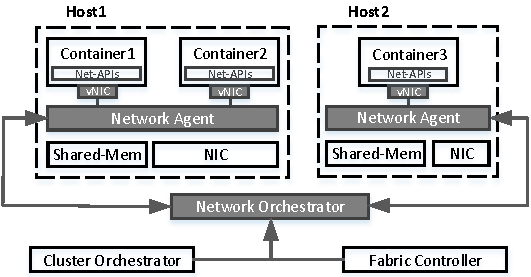
\includegraphics[width=7in]{figures/system-arch.pdf} 
    \caption{\label{fig:sysarch} The overall system architecture of exsiting overlay network and \sysname. Gray boxes are building blocks of~\sysname.} 
\end{figure*} 

In this section, we discuss the key insights to achieve a high network
performance without sacrificing portability of containers. We also 
introduce the overall architecture of \sysname. 

%This section presents the high-level design of \sysname. We introduce
%the requirements and concerns in the designs of control-plane, data-plane
%and network access layer, and explain what design choices \sysname makes 
%and what the reasons are behind these design choices.

\subsection{Portability v.s. Performance}
Container deployments opt for overlay-based networking since it is most
portable: a container does not have to worry about where the other endpoint is.
For example, in Figure~\ref{fig:overlay}, Container~1 and Container~3 cannot
distinguish whether Container~2 is on Host~1 or Host~2, if only Container~2
keeps its overlay IP address (2.2.2.2) and the overlay routers know how to
route packets to this IP. 

Existing overlay-based container networks sacrifice performance for 
the good portability, because traffic needs to go through a deep software 
stack, including bridges, routers and host OS kernels. 
The key to achieve a high performance and low overhead overlay network for
containers is bypassing the performance bottlenecks, including bridges, software
routers and host OS kernel, on data-plane. Given that containers are essentially
processes, the communication channels provided by IPC and hardware offloading
techniques give us numerous hammers to build a better container network. For
instance, containers within a single host (like Container~1 and Container~2 in
Figure~\ref{fig:overlay}) can communicate via shared-memory, and software routers
in different hosts can talk via RDMA (or DPDK), which helps to bypass performance
bottlenecks. In other words, one container should decide how to communicate
with another according to the latter's location. 

\subsection{Our approach}

To bypass bottlenecks and get high network performance on overlay
networks, there are two issues to solve: (1) How to discover the real-time locations of containers; (2) How to enable containers
to use different mechanisms to communicate with different peers.

One way is to solve these two issues merely depending on containers themselves:
one container needs to exchange location information with the other first and
agree on a communication mechanism to use. Nonetheless, this method will 
break the portability of containers, e.g. container locations are never transparent, and will also make the programing of applications extremely 
complicated. 

Instead, we take an alternative approach: using a centralized orchestrator to decide how containers communicate, and keeping the container locations and the actual
communication mechanisms transparent to containers.
Our key insight is that since currently most of the container clusters are managed by a centralized cluster orchestrator, the information about the location of the other endpoint
can be easily obtained by querying the orchestrator. By leveraging this
information, we can choose the right communication paradigm for the specific
scenario. Furthermore, all of this complexity can be hidden from the application
by bundling it into a virtual interface, and associated code. Next, we sketch the architecture of our solution.

\subsection{The architecture of FreeFlow}

